\documentclass{beamer}
\usepackage{amsmath,graphics}
\usepackage{amssymb}

\usetheme{default}
\usepackage{xcolor}

\definecolor{solarizedBase03}{HTML}{002B36}
\definecolor{solarizedBase02}{HTML}{073642}
\definecolor{solarizedBase01}{HTML}{586e75}
\definecolor{solarizedBase00}{HTML}{657b83}
\definecolor{solarizedBase0}{HTML}{839496}
\definecolor{solarizedBase1}{HTML}{93a1a1}
\definecolor{solarizedBase2}{HTML}{EEE8D5}
\definecolor{solarizedBase3}{HTML}{FDF6E3}
\definecolor{solarizedYellow}{HTML}{B58900}
\definecolor{solarizedOrange}{HTML}{CB4B16}
\definecolor{solarizedRed}{HTML}{DC322F}
\definecolor{solarizedMagenta}{HTML}{D33682}
\definecolor{solarizedViolet}{HTML}{6C71C4}
%\definecolor{solarizedBlue}{HTML}{268BD2}
\definecolor{solarizedBlue}{HTML}{134676}
\definecolor{solarizedCyan}{HTML}{2AA198}
\definecolor{solarizedGreen}{HTML}{859900}
\definecolor{myBlue}{HTML}{162DB0}%{261CA4}
\setbeamercolor*{item}{fg=myBlue}
\setbeamercolor{normal text}{fg=solarizedBase03, bg=solarizedBase3}
\setbeamercolor{alerted text}{fg=myBlue}
\setbeamercolor{example text}{fg=myBlue, bg=solarizedBase3}
\setbeamercolor*{frametitle}{fg=solarizedRed}
\setbeamercolor*{title}{fg=solarizedRed}
\setbeamercolor{block title}{fg=myBlue, bg=solarizedBase3}
\setbeameroption{hide notes}
\setbeamertemplate{note page}[plain]
\beamertemplatenavigationsymbolsempty
\usefonttheme{professionalfonts}
\usefonttheme{serif}

\usepackage{fourier}

\def\vec#1{\mathchoice{\mbox{\boldmath$\displaystyle#1$}}
{\mbox{\boldmath$\textstyle#1$}}
{\mbox{\boldmath$\scriptstyle#1$}}
{\mbox{\boldmath$\scriptscriptstyle#1$}}}
\definecolor{OwnGrey}{rgb}{0.560,0.000,0.000} % #999999
\definecolor{OwnBlue}{rgb}{0.121,0.398,0.711} % #1f64b0
\definecolor{red4}{rgb}{0.5,0,0}
\definecolor{blue4}{rgb}{0,0,0.5}
\definecolor{Blue}{rgb}{0,0,0.66}
\definecolor{LightBlue}{rgb}{0.9,0.9,1}
\definecolor{Green}{rgb}{0,0.5,0}
\definecolor{LightGreen}{rgb}{0.9,1,0.9}
\definecolor{Red}{rgb}{0.9,0,0}
\definecolor{LightRed}{rgb}{1,0.9,0.9}
\definecolor{White}{gray}{1}
\definecolor{Black}{gray}{0}
\definecolor{LightGray}{gray}{0.8}
\definecolor{Orange}{rgb}{0.1,0.2,1}
\setbeamerfont{sidebar right}{size=\scriptsize}
\setbeamercolor{sidebar right}{fg=Black}

\renewcommand{\emph}[1]{{\textcolor{solarizedRed}{\itshape #1}}}

\newcommand\cA{\mathcal A}
\newcommand\cB{\mathcal B}
\newcommand\cC{\mathcal C}
\newcommand\cD{\mathcal D}
\newcommand\cE{\mathcal E}
\newcommand\cF{\mathcal F}
\newcommand\cG{\mathcal G}
\newcommand\cH{\mathcal H}
\newcommand\cI{\mathcal I}
\newcommand\cJ{\mathcal J}
\newcommand\cK{\mathcal K}
\newcommand\cL{\mathcal L}
\newcommand\cM{\mathcal M}
\newcommand\cN{\mathcal N}
\newcommand\cO{\mathcal O}
\newcommand\cP{\mathcal P}
\newcommand\cQ{\mathcal Q}
\newcommand\cR{\mathcal R}
\newcommand\cS{\mathcal S}
\newcommand\cT{\mathcal T}
\newcommand\cU{\mathcal U}
\newcommand\cV{\mathcal V}
\newcommand\cW{\mathcal W}
\newcommand\cX{\mathcal X}
\newcommand\cY{\mathcal Y}
\newcommand\cZ{\mathcal Z}

\newcommand\fA{\mathfrak A}
\newcommand\fB{\mathfrak B}
\newcommand\fC{\mathfrak C}
\newcommand\fD{\mathfrak D}
\newcommand\fE{\mathfrak E}
\newcommand\fF{\mathfrak F}
\newcommand\fG{\mathfrak G}
\newcommand\fH{\mathfrak H}
\newcommand\fI{\mathfrak I}
\newcommand\fJ{\mathfrak J}
\newcommand\fK{\mathfrak K}
\newcommand\fL{\mathfrak L}
\newcommand\fM{\mathfrak M}
\newcommand\fN{\mathfrak N}
\newcommand\fO{\mathfrak O}
\newcommand\fP{\mathfrak P}
\newcommand\fQ{\mathfrak Q}
\newcommand\fR{\mathfrak R}
\newcommand\fS{\mathfrak S}
\newcommand\fT{\mathfrak T}
\newcommand\fU{\mathfrak U}
\newcommand\fV{\mathfrak V}
\newcommand\fW{\mathfrak W}
\newcommand\fX{\mathfrak X}
\newcommand\fY{\mathfrak Y}
\newcommand\fZ{\mathfrak Z}

\newcommand\fa{\mathfrak a}
\newcommand\fb{\mathfrak b}
\newcommand\fc{\mathfrak c}
\newcommand\fd{\mathfrak d}
\newcommand\fe{\mathfrak e}
\newcommand\ff{\mathfrak f}
\newcommand\fg{\mathfrak g}
\newcommand\fh{\mathfrak h}
%\newcommand\fi{\mathfrak i}
\newcommand\fj{\mathfrak j}
\newcommand\fk{\mathfrak k}
\newcommand\fl{\mathfrak l}
\newcommand\fm{\mathfrak m}
\newcommand\fn{\mathfrak n}
\newcommand\fo{\mathfrak o}
\newcommand\fp{\mathfrak p}
\newcommand\fq{\mathfrak q}
\newcommand\fr{\mathfrak r}
\newcommand\fs{\mathfrak s}
\newcommand\ft{\mathfrak t}
\newcommand\fu{\mathfrak u}
\newcommand\fv{\mathfrak v}
\newcommand\fw{\mathfrak w}
\newcommand\fx{\mathfrak x}
\newcommand\fy{\mathfrak y}
\newcommand\fz{\mathfrak z}

\newcommand\vA{\vec A}
\newcommand\vB{\vec B}
\newcommand\vC{\vec C}
\newcommand\vD{\vec D}
\newcommand\vE{\vec E}
\newcommand\vF{\vec F}
\newcommand\vG{\vec G}
\newcommand\vH{\vec H}
\newcommand\vI{\vec I}
\newcommand\vJ{\vec J}
\newcommand\vK{\vec K}
\newcommand\vL{\vec L}
\newcommand\vM{\vec M}
\newcommand\vN{\vec N}
\newcommand\vO{\vec O}
\newcommand\vP{\vec P}
\newcommand\vQ{\vec Q}
\newcommand\vR{\vec R}
\newcommand\vS{\vec S}
\newcommand\vT{\vec T}
\newcommand\vU{\vec U}
\newcommand\vV{\vec V}
\newcommand\vW{\vec W}
\newcommand\vX{\vec X}
\newcommand\vY{\vec Y}
\newcommand\vZ{\vec Z}

\newcommand\va{\vec a}
\newcommand\vb{\vec b}
\newcommand\vc{\vec c}
\newcommand\vd{\vec d}
\newcommand\ve{\vec e}
\newcommand\vf{\vec f}
\newcommand\vg{\vec g}
\newcommand\vh{\vec h}
\newcommand\vi{\vec i}
\newcommand\vj{\vec j}
\newcommand\vk{\vec k}
\newcommand\vl{\vec l}
\newcommand\vm{\vec m}
\newcommand\vn{\vec n}
\newcommand\vo{\vec o}
\newcommand\vp{\vec p}
\newcommand\vq{\vec q}
\newcommand\vr{\vec r}
\newcommand\vs{\vec s}
\newcommand\vt{\vec t}
\newcommand\vu{\vec u}
\newcommand\vv{\vec v}
\newcommand\vw{\vec w}
\newcommand\vx{\vec x}
\newcommand\vy{\vec y}
\newcommand\vz{\vec z}

\renewcommand\AA{\mathbb A}
\newcommand\NN{\mathbb N}
\newcommand\ZZ{\mathbb Z}
\newcommand\PP{\mathbb P}
\newcommand\QQ{\mathbb Q}
\newcommand\RR{\mathbb R}
\renewcommand\SS{\mathbb S}
\newcommand\CC{\mathbb C}

\newcommand{\ord}{\mathrm{ord}}
\newcommand{\id}{\mathrm{id}}
\newcommand{\pr}{\mathrm{P}}
\newcommand{\Vol}{\mathrm{vol}}
\newcommand\norm[1]{\left\|{#1}\right\|} 
\newcommand\sign{\mathrm{sign}}
\newcommand{\eps}{\varepsilon}
\newcommand{\abs}[1]{\left|#1\right|}
\newcommand\bc[1]{\left({#1}\right)} 
\newcommand\cbc[1]{\left\{{#1}\right\}} 
\newcommand\bcfr[2]{\bc{\frac{#1}{#2}}} 
\newcommand{\bck}[1]{\left\langle{#1}\right\rangle} 
\newcommand\brk[1]{\left\lbrack{#1}\right\rbrack} 
\newcommand\scal[2]{\bck{{#1},{#2}}} 
\newcommand{\vecone}{\mathbb{1}}
\newcommand{\tensor}{\otimes}
\newcommand{\diag}{\mathrm{diag}}
\newcommand{\ggt}{\mathrm{ggT}}
\newcommand{\kgv}{\mathrm{kgV}}

\newcommand{\Karonski}{Karo\'nski}
\newcommand{\Erdos}{Erd\H{o}s}
\newcommand{\Renyi}{R\'enyi}
\newcommand{\Lovasz}{Lov\'asz}
\newcommand{\Juhasz}{Juh\'asz}
\newcommand{\Bollobas}{Bollob\'as}
\newcommand{\Furedi}{F\"uredi}
\newcommand{\Komlos}{Koml\'os}
\newcommand{\Luczak}{\L uczak}
\newcommand{\Kucera}{Ku\v{c}era}
\newcommand{\Szemeredi}{Szemer\'edi}

\renewcommand{\ae}{\"a}
\renewcommand{\oe}{\"o}
\newcommand{\ue}{\"u}
\newcommand{\Ae}{\"A}
\newcommand{\Oe}{\"O}
\newcommand{\Ue}{\"U}

\title[Linadi]{Abelsche Gruppen}
\author[Amin Coja-Oghlan]{Amin Coja-Oghlan}
\institute[Frankfurt]{JWGUFFM}
\date{}

\begin{document}

\frame[plain]{\titlepage}

\begin{frame}\frametitle{Abelsche Gruppen}
	\begin{block}{Erinnerung}
		Eine \emph{Gruppe} ist eine Menge $G$ zusammen mit einer Abbildung 
		\begin{align*}
			*:G\times G\to G,&&(x,y)\mapsto x*y
		\end{align*}
 die folgende Bedingungen erf\"ullt:
		\begin{description}
			\item[Assoziativgesetz:] f\ue r alle $x,y,z\in G$ gilt $$(x*y)*z=x*(y*z).$$
			\item[Neutrales Element:] es gibt ein $e\in G$, so da\ss\ f\ue r alle $x\in G$ gilt $$e*x=x.$$
			\item[Inverses Element:] zu jedem $x\in G$ gibt es ein $y\in G$ mit $$y*x=e.$$
		\end{description}
	\end{block}
\end{frame}

\begin{frame}\frametitle{Abelsche Gruppen}
	\begin{block}{Definition}
		Eine Gruppe $(G,*)$ hei\ss t \emph{Abelsch}, falls
		\begin{align*}
			x*y=y*x&&\mbox{f\ue r alle }x,y\in G.
		\end{align*}
	\end{block}
\end{frame}

\begin{frame}\frametitle{Abelsche Gruppen}
	\begin{block}{Beispiele}
	\begin{itemize}
		\item Die Gruppe $(\ZZ,+)$ ist Abelsch
		\item Die Gruppe $(\QQ\setminus\cbc 0,\,\cdot\,)$ ist Abelsch.
		\item Die Kleinsche Vierergruppe ist Abelsch.
		\item Die Symmetrische Gruppe $\SS_3$ ist \emph{nicht} Abelsch.
	\end{itemize}
	\end{block}
\end{frame}

\begin{frame}\frametitle{Die zyklische Gruppe}
	\begin{overprint}
		\onslide<1>
		\begin{block}{Definition}
			Seien $A,B\subseteq\QQ$. 
			\begin{itemize}
				\item Mit $A+B$ bezeichnen wir die Menge
					\begin{align*}
						\cbc{a+b:a\in A,\,b\in B}.
					\end{align*}
				\item Mit $A\cdot B$ bezeichnen wir die Menge
					\begin{align*}
						\cbc{a\cdot b:a\in A,b\in B}.
					\end{align*}
				\item F\ue r $x\in\QQ$ bezeichen definieren wir
					\begin{align*}
						x+A=\{x\}+A=\{x+a:a\in A\}.
					\end{align*}
				\item F\ue r $x\in\QQ$ bezeichen definieren wir
					\begin{align*}
						x\cdot A=\{x\}\cdot A=\{x\cdot a:a\in A\}.
					\end{align*}
			\end{itemize}
		\end{block}	
		\onslide<2>
		\begin{block}{Definition}
			\begin{itemize}
				\item Sei $n\in\NN$.
				\item Es sei
					\begin{align*}
						\ZZ_n=\cbc{z+n\cdot\ZZ:z\in\ZZ}.
					\end{align*}
				\item Wir definieren auf $\ZZ_n$ eine Verkn\ue pfung $+$ durch
					\begin{align*}
						(x+n\cdot\ZZ)+(y+n\cdot\ZZ)=(x+y)+n\cdot\ZZ.
					\end{align*}
			\end{itemize}
		\end{block}
	\end{overprint}
\end{frame}

\begin{frame}\frametitle{Die zyklische Gruppe}
	\begin{overprint}
		\onslide<1>
		\begin{block}{Beispiel $\ZZ_2$}
			\begin{itemize}
				\item Es ist
					\begin{align*}
						2\cdot\ZZ&=\{2\cdot z:z\in\ZZ\}=\{0,\pm2,\pm4,\pm6,\pm8\ldots\}\\
								 &=\{\ldots,-8,-6,-4,-2,0,2,4,6,8,\ldots\}
					\end{align*}
				\item Ferner
					\begin{align*}
						0+2\cdot\ZZ&=\{0+2\cdot z:z\in\ZZ\}=\{\ldots,-8,-6,-4,-2,0,2,4,6,8,\ldots\}\\
						1+2\cdot\ZZ&=\{1+2\cdot z:z\in\ZZ\}=\{\ldots,-7,-5,-3,-1,1,3,5,7,9,\ldots\}\\
						2+2\cdot\ZZ&=\{2+2\cdot z:z\in\ZZ\}=\{\ldots,-6,-4,-2,0,2,4,6,8,10,\ldots\}=2\cdot\ZZ\\
						3+2\cdot\ZZ&=\{3+2\cdot z:z\in\ZZ\}=\{\ldots,-5,-3,-1,1,3,5,7,9,11\ldots\}=1+2\cdot\ZZ\\
					\end{align*}
			\end{itemize}
		\end{block}
		\onslide<2>
		\begin{block}{Beispiel $\ZZ_2$}
			\begin{itemize}
				\item Entsprechend
					\begin{align*}
						-1+2\cdot\ZZ&=\{\ldots,-9,-7,-5,-3,-1,1,3,5,7,\ldots\}=1+2\cdot\ZZ\\
						-2+2\cdot\ZZ&=\{\ldots,-10,-8,-6,-4,-2,0,2,4,6,\ldots\}=2\cdot\ZZ\\
						-3+2\cdot\ZZ&=\{\ldots,-11,-9,-7,-5,-3,-1,1,3,5,\ldots\}=1+2\cdot\ZZ
					\end{align*}
				\item Also
					\begin{align*}
						z+2\cdot\ZZ=\begin{cases}
							2\cdot\ZZ&\mbox{ falls $z$ gerade}\\
							1+2\cdot\ZZ&\mbox{ falls $z$ ungerade}
						\end{cases}
					\end{align*}
			\end{itemize}
		\end{block}
		\onslide<3>
		\begin{block}{Beispiel $\ZZ_2$}
			\begin{itemize}
				\item Folglich hat $\ZZ_2$ genau die zwei Elemente
					\begin{align*}
						\ZZ_2=\cbc{0+2\ZZ,1+2\ZZ}.
					\end{align*}
				\item Die $+$-Operation ist definiert durch die Tabelle
					\begin{align*}
						\begin{array}{c|c|c}
							+&0+2\ZZ&1+2\ZZ\\\hline
							0+2\ZZ&0+2\ZZ&1+2\ZZ\\\hline
							1+2\ZZ&1+2\ZZ&0+2\ZZ
						\end{array}	
					\end{align*}
				\item Also ist $(\ZZ_2,+)$ eine Abelsche Gruppe
				\item Neutrales Element ist $0+2\ZZ$.
			\end{itemize}
		\end{block}
	\end{overprint}
\end{frame}

\begin{frame}\frametitle{Die zyklische Gruppe}
	\begin{overprint}
		\onslide<1>
		\begin{block}{Beispiel $\ZZ_3$}
			\begin{itemize}
				\item Es ist
					\begin{align*}
						3\cdot\ZZ&=\{3\cdot z:z\in\ZZ\}=\{0,\pm3,\pm6,\pm9,\pm12\ldots\}\\
								 &=\{\ldots,-8,-6,-4,-2,0,2,4,6,8,\ldots\}
					\end{align*}
				\item Ferner
					\begin{align*}
						0+3\cdot\ZZ&=\{\ldots,-9,-6,-3,0,3,6,9,\ldots\}\\
						1+3\cdot\ZZ&=\{\ldots,-8,-5,-2,1,4,7,10,\ldots\}\\
						2+3\cdot\ZZ&=\{\ldots,-7,-4,-1,2,5,8,11,\ldots\}\\
						3+3\cdot\ZZ&=\{\ldots,-6,-3,0,3,6,9,12,\ldots\}=3\cdot\ZZ\\
						4+3\cdot\ZZ&=\{\ldots,-5,-2,1,4,7,10,13,\ldots\}=1+3\cdot\ZZ\\
						5+3\cdot\ZZ&=\{\ldots,-4,-1,2,5,8,11,14,\ldots\}=2+3\cdot\ZZ\\
					\end{align*}
			\end{itemize}
		\end{block}
		\onslide<2>
		\begin{block}{Beispiel $\ZZ_3$}
			\begin{itemize}
				\item Analog
					\begin{align*}
						0+3\cdot\ZZ&=\{\ldots,-9,-6,-3,0,3,6,9,\ldots\}\\
						-1+3\cdot\ZZ&=\{\ldots,-10,-7,-4,-1,2,5,8,\ldots\}\\
						-2+3\cdot\ZZ&=\{\ldots,-11,-8,-5,-2,1,4,7,\ldots\}\\
						-3+3\cdot\ZZ&=\{\ldots,-12,-9,-6,-3,0,3,6,\ldots\}=3\cdot\ZZ\\
						-4+3\cdot\ZZ&=\{\ldots,-13,-10,-7,-4,-1,2,5,\ldots\}=2+3\cdot\ZZ\\
						-5+3\cdot\ZZ&=\{\ldots,-14,-11,-8,-5,-2,1,4,\ldots\}=1+3\cdot\ZZ
					\end{align*}
				\item Also $\displaystyle z+3\cdot\ZZ=\begin{cases} 3\cdot\ZZ&\mbox{ falls $z\equiv0\mod3$}\\ 1+3\cdot\ZZ&\mbox{ falls $z\equiv1\mod3$}\\2+3\cdot\ZZ&\mbox{ falls $z\equiv2\mod3$} \end{cases} $
			\end{itemize}
		\end{block}
		\onslide<3>
		\begin{block}{Beispiel $\ZZ_3$}
			\begin{itemize}
				\item Folglich hat $\ZZ_3$ genau die drei Elemente
					\begin{align*}
						\ZZ_3=\cbc{0+3\ZZ,1+3\ZZ,2+3\ZZ}.
					\end{align*}
				\item Die $+$-Operation ist definiert durch die Tabelle
					\begin{align*}
						\begin{array}{c|c|c|c}
							+&0+3\ZZ&1+3\ZZ&2+3\ZZ\\\hline
							0+3\ZZ&0+3\ZZ&1+3\ZZ&2+3\ZZ\\\hline
							1+3\ZZ&1+3\ZZ&2+3\ZZ&0+3\ZZ\\\hline
							2+3\ZZ&2+3\ZZ&0+3\ZZ&1+3\ZZ
						\end{array}	
					\end{align*}
				\item Also ist $(\ZZ_3,+)$ eine Abelsche Gruppe
				\item Neutrales Element ist $0+3\ZZ$.
			\end{itemize}
		\end{block}
	\end{overprint}
\end{frame}


\begin{frame}\frametitle{Die zyklische Gruppe}
	\begin{block}{Rechnen in $\ZZ_n$}
		\begin{itemize}
			\item Allgemein hat die Gruppe $\ZZ_n$ die $n$ Elemente
				\begin{align*}
					\ZZ_n&=\{0+n\ZZ,1+n\ZZ,2+n\ZZ,\ldots,(n-1)+n\ZZ\}.
				\end{align*}
			\item Es gilt $x+n\ZZ=y+n\ZZ$ genau dann, wenn
				\begin{align*}
					x\equiv y\mod n.
				\end{align*}
		\end{itemize}
	\end{block}
\end{frame}

\begin{frame}\frametitle{Die zyklische Gruppe}
	\begin{block}{Rechnen in $\ZZ_n$}
		Um $(x+n\ZZ)+(y+n\ZZ)$ zu berechnen, gehen wir wie folgt vor:
		\begin{itemize}
			\item Bestimme $z=x+y$.
			\item Teile $z$ mit Rest durch $n$:
				\begin{align*}
					z&=q\cdot n+r&&\mbox{mit }0\leq r<n.
				\end{align*}
			\item Das Ergebnis ist dann $r+n\ZZ$, also
				\begin{align*}
					(x+n\ZZ)+(y+n\ZZ)=r+n\ZZ.
				\end{align*}
		\end{itemize}	
	\end{block}
\end{frame}

\begin{frame}\frametitle{Die zyklische Gruppe}
	\begin{block}{Beispiel: $\ZZ_6$}
		\centering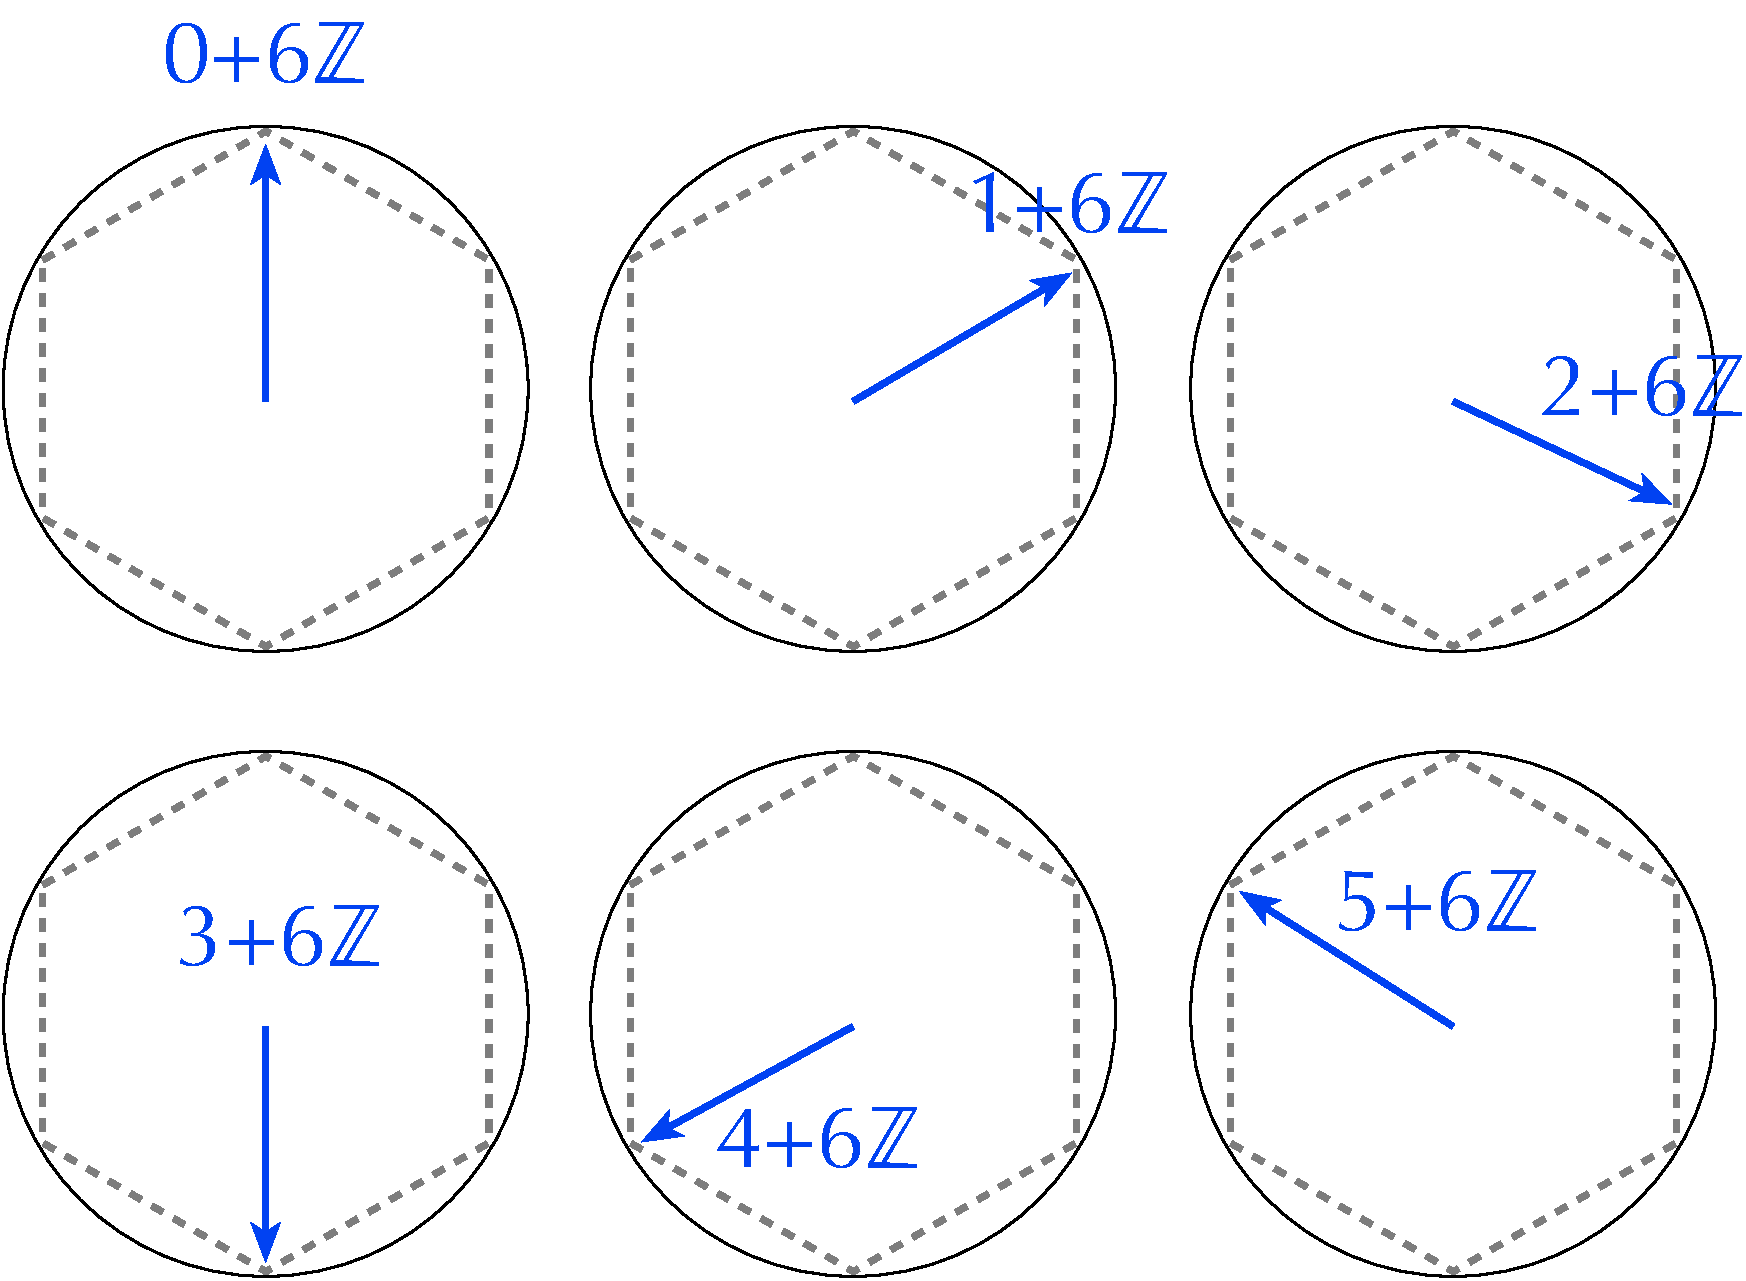
\includegraphics[width=100mm]{pics/cyclicGroup.pdf}
	\end{block}
\end{frame}

\begin{frame}\frametitle{Die zyklische Gruppe}
	\begin{block}{Beispiel: $\ZZ_6$}
		\centering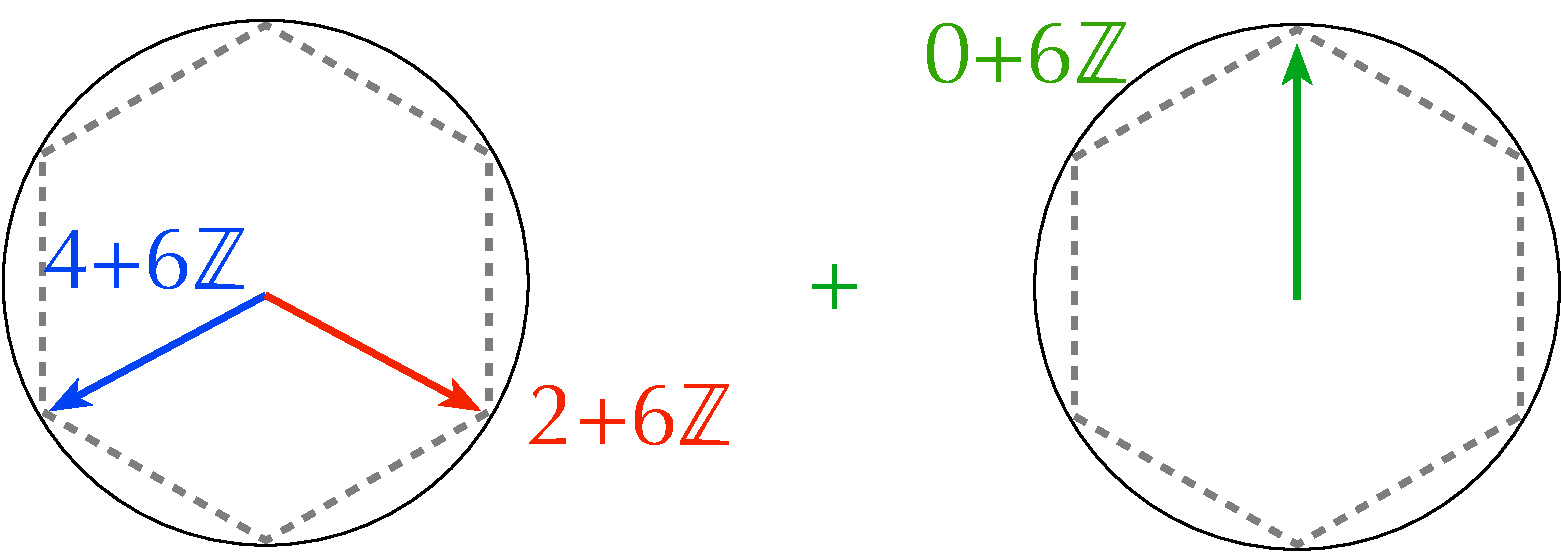
\includegraphics[width=100mm]{pics/cyclicGroup1.pdf}
	\end{block}
\end{frame}

\begin{frame}\frametitle{Die zyklische Gruppe}
	\begin{block}{Beispiel: $\ZZ_6$}
		\centering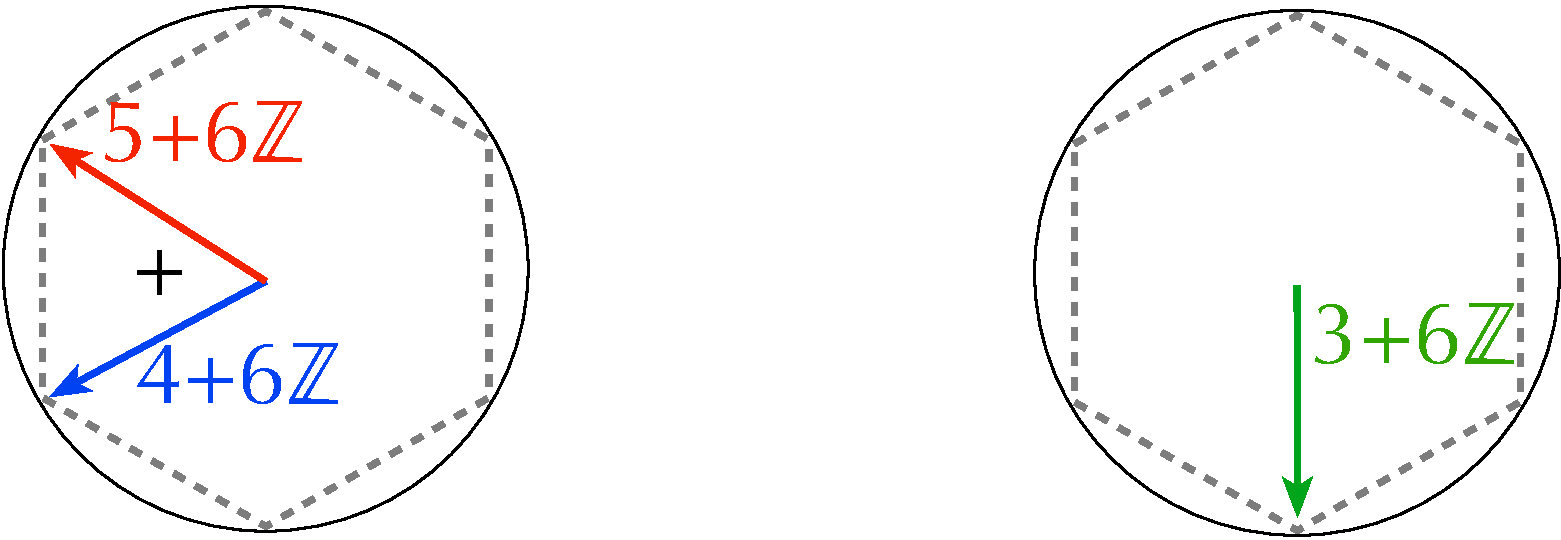
\includegraphics[width=100mm]{pics/cyclicGroup2.pdf}
	\end{block}
\end{frame}

\begin{frame}\frametitle{Die zyklische Gruppe}
	\begin{block}{Lemma}
		In der zyklischen Gruppe $\ZZ_n$ hat $1+n\ZZ$ die Ordnung $n$.
	\end{block}
	\begin{block}{Beweis}
		\begin{itemize}
			\item Wir wissen bereits, da\ss\ $\ord_{\ZZ_n}(1+\ZZ_n)\leq n$.
			\item Umgekehrt gilt nach der Rechenregel f\ue r $\ZZ_n$:
				\begin{align*}
					\underbrace{(1+n\ZZ)+\cdots+(1+n\ZZ)}_{\mbox{$i$ mal}}\neq0+n\ZZ\qquad\mbox{f\ue r }1\leq i<n.
				\end{align*}
			\item Also gilt $\ord_{\ZZ_n}(1+\ZZ_n)\geq n$
		\end{itemize}
	\end{block}
\end{frame}

\begin{frame}\frametitle{Gruppenisomorphismen}
	\begin{overprint}
		\onslide<1>
		\begin{block}{Definition}
			Seien $(G,*)$, $(H,\star)$ Gruppen.
			Ein bijektiver Homomorphismus $f:G\to H$ hei\ss t ein \emph{Isomorphismus}.
		\end{block}
		\onslide<2>
		\begin{block}{Anmerkung}
			\begin{itemize}
				\item Eine Isomorphismus $f:G\to H$ hat die Eigenschaft
					\begin{align*}
						f(x*y)&=f(x)\star f(y)&&\mbox{f\ue r alle }x,y\in G\\
						f^{-1}(u)*f^{-1}(v)&=u\star v&&\mbox{f\ue r alle }u,v\in H
					\end{align*}
				\item Wenn es einen Isomorphismus gibt, unterscheiden sich die Gruppen nur in der Benennung der Elemente und der Gruppenoperation.
				\item In diesem Fall schreibt man $G\cong H$.
			\end{itemize}
		\end{block}
	\end{overprint}
\end{frame}

\begin{frame}\frametitle{Gruppenisomorphismen}
	\begin{block}{Definition}
		Eine endliche Gruppe $G$ hei\ss t \emph{zyklisch}, wenn es eine Zahl $n\in\NN$ gibt, so da\ss\
		\begin{align*}
			G\cong \ZZ_n.
		\end{align*}
	\end{block}
\end{frame}

\begin{frame}\frametitle{Gruppenisomorphismen}
	\begin{block}{Anmerkung}
		\begin{itemize}
			\item Jede zyklische Gruppe ist Abelsch.
			\item Es gibt aber Abelsche Gruppen, die nicht zyklisch sind.
			\item Beispiel: Kleinsche Vierergruppe.
		\end{itemize}
	\end{block}
\end{frame}

\begin{frame}\frametitle{Zusammenfassung}
	\begin{itemize}
		\item Definition Abelsche Gruppe
		\item Die zyklische Gruppe $\ZZ_n$
		\item Gruppenisomorphismen
	\end{itemize}
\end{frame}

\end{document}
